\documentclass{article}
\usepackage[utf8]{inputenc}
\usepackage[english, swedish]{babel}

\usepackage{cite}
\usepackage{caption}
\usepackage{graphicx}
\usepackage{float}
\usepackage{textcomp}
\usepackage[yyyymmdd]{datetime}
\renewcommand{\dateseparator}{-}

\usepackage{graphicx}
\graphicspath{ {images/} }

%For headers & footers
\usepackage{fancyhdr}
\pagestyle{fancy}
\lhead{
\includegraphics[scale=0.2]{Logo}}
\chead{Kartrobot}
\rhead{\today}

\lfoot{Konstruktion med mikrodatorer}
\rfoot{Grupp 3}

\renewcommand{\headrulewidth}{0.4pt}
\renewcommand{\footrulewidth}{0.4pt}


\title{Teknisk dokumentation för kartrobot}
\author{Patrik Sletmo}
\date{\today}

\selectlanguage{swedish}

\begin{document}

\thispagestyle{empty}

{
\sffamily
\centering
\large


{\huge 
Designspecifikation för kartrobot
}

{\large
Patrik Sletmo
}

{\large
Version 1.0
}

\vspace{3.5cm}

Status
\begin{table}[H]
\centering
\begin{tabular}{ | c | c | c | }
\hline
STATUS & Patrik Sletmo & 2016-12-DD \\
\hline
\end{tabular}
\end{table}
}
\clearpage

\vspace*{\fill}
{
\sffamily
\centering
\large


{\huge
Projektidentitet
}

{\large
Grupp 3, 16/HT, KarToffel \\ Linköpings tekniska högskola, ISY
}

\vspace{0.5cm}

\begin{table}[H]
\centering
\begin{tabular}{ | c | c | c | c |}
\hline
Namn & Ansvar & Telefon & E-post \\
\hline
Patrik Sletmo & Projektledare & 070 783 57 61 & patsl736@student.liu.se \\
\hline
Rebecca Lindblom & Utvecklare & 073 436 40 79 & rebli156@student.liu.se \\
\hline
Matildha Sjöstedt & Utvecklare & 070 515 84 11 & matsj696@student.liu.se \\
\hline
Sebastian Callh & Utvecklare & 073 820 46 64 & sebca553@student.liu.se \\
\hline
Anton Dalgren & Utvecklare & 076 836 51 56 & antda685@student.liu.se \\
\hline
Matilda Dahlström & Utvecklare & 070 636 33 52 & matda715@student.liu.se \\
\hline
\end{tabular}
\end{table}
}

\begin{center}
\textbf{Hemsida}: https://github.com/SebastianCallh/kartoffel-tsea29
\end{center}

\begin{center}
\textbf{Kund}: Mattias Krysander, 013 - 28 2198 , matkr@isy.liu.se
\end{center}

\begin{center}
\textbf{Kursansvarig}: Tomas Svensson, 3B 528, +46 (0)13 28 1368, tomas.svensson@liu.se \\
\textbf{Handledare}: Anders Nilsson, 3B 512, +46 (0)13 28 2635, anders.p.nilsson@liu.se
\end{center}
\vspace*{\fill}
\clearpage

\renewcommand*\contentsname{Innehållsförteckning}
\tableofcontents
\clearpage


{
\sffamily
\centering
\large


{\huge 
Dokumenthistorik \\
}
\begin{table}[H]
\centering
\begin{tabular}{ | c | c | c | c | c |} 
\hline
\textbf{Version} & \textbf{Datum} & \textbf{Utförda ändringar} & \textbf{Utförd av } & \textbf{Granskad} \\
\hline
VERSION & 2016-12-DD & Första version & Grupp 3 & Patrik Sletmo \\
\hline

\end{tabular}
\end{table}
}

\section{Inledning}
% Kort beskrivning av hela dokumentet, skrivs förslagsvis sist

\section{Systembeskrivning}
% Beskrivning av systemets mest framträdande egenskaper

\subsection{Delsystem}
% Upplistning av delsystem, eventuellt någon kort kommentar om varje delsystem
Hela systemet är moduluppbyggt, och består av följande delsystem:
\begin{itemize}
\item Mjuvaruenhet
\item Huvudenhet
\item Sensorenhet
\item Styrenhet
\end{itemize}

\subsection{Övergripande konstruktion}
% Övergripande blockschema
\begin{figure}[H]
\centering

\includegraphics[scale=0.4]{Logo}
\caption{Översikt över systemet}
\label{fig:oversikt_systemet3}
\end{figure}

TODO:TEXT OM ÖVERGRIPANDE KONSTRUKTION OCH FIGUR

\subsection{Komponenter}
% Väldigt kort beskrivning av delsektion
Här nedan listas alla komponenter som roboten består av.

\subsubsection{Beräkningsenheter}
% Upplistning av processorer, SOC:s, etc
\begin{table}[H]
  \centering
  \begin{tabular}{ | c | c | c | c |}
    \hline
    \textbf{Enhet} & \textbf{Antal} \\
    \hline
    Raspberry Pi 3 & 1 \\
    \hline
    ATMega 1284 & 2 \\
    \hline
  \end{tabular}
  \caption{ Tabell över beräkningsenheter. }
\end{table}

\subsubsection{Sensorer}
% Upplistning av alla sensorer
\begin{table}[H]
  \centering
  \begin{tabular}{ | c | c | c | c |}
    \hline
    \textbf{Komponent} & \textbf{Antal} \\
    \hline
    LIDAR-Lite v2 & 1 \\
    \hline
    Knapp & 1 \\
    \hline
    GP2Y0A41SK IR-Sensor & 2 \\
    \hline
    GP2Y0A21 IR-Sensor & 1 \\
    \hline
    Adafruit 10-DOF IMU & 2 \\
    \hline
  \end{tabular}
  \caption{ Tabell över sensorer. }
\end{table}

\subsubsection{Ställdon}
% Servon, motorer, etc
\begin{table}[H]
  \centering
  \begin{tabular}{ | c | c | c | c |}
    \hline
    \textbf{Komponent} & \textbf{Antal} \\
    \hline
    291RPM DC-motor & 4 \\
    \hline
  \end{tabular}
  \caption{ Tabell över ställdon. }
\end{table}

TODO:TABELL NEDAN EJ KORRIGERAD
\subsubsection{IC-kretsar}
% Shifters
\begin{table}[H]
  \centering
  \begin{tabular}{ | c | c | c | c |}
    \hline
    \textbf{Komponent} & \textbf{Antal} \\
    \hline
    BSS138 & 1 \\
   \hline
    EXO3 & 1 \\
    \hline
    LS241 & 1 \\
    \hline
  \end{tabular}
  \caption{ Tabell över IC-kretsar. }
\end{table}

\clearpage
\section{Delsystem}

\subsection{Huvudenhet}
TODO:TEXT OM HUVUDENHET

\subsubsection{Delsystemets funktion}
TODO:TEXT OM DELSYSTEMETS FUNKTION

\subsubsection{Kopplingsschema}
\begin{figure}[H]
\centering

\includegraphics[scale=0.45]{Logo}
\caption{Kopplingsschema för huvudenheten.}
\label{fig:huvudenhet_kopplingsschema}
\end{figure}

TODO:TEXT OM KOPPLINGSCHEMAT

\subsubsection{Komponenter}

\begin{table}[H]
   \centering
  \begin{tabular}{ | c | c | }
    \hline
    \textbf{Komponent} & \textbf{Antal} \\
    \hline
    Raspberry PI 3 & 1 \\
    \hline
    BSS138 & 2 \\
    \hline
  \end{tabular}
\end{table}

\subsubsection{Resurser}

TODO:TABELLEN NEDAN EJ KORRIGERAD
\begin{table}[H]
   \centering
  \begin{tabular}{ | c | c | c | }
    \hline
    \textbf{Port} & \textbf{Antal} & \textbf{Används} \\
    \hline
    GPIO pins & 40 & 2 \\
    \hline
  \end{tabular}
\end{table}


\subsubsection{Programflöde}
Programflödet i huvudenheten består i huvudsak av två delar: Den logiska delen som sköter navigeringsbesluten utifrån beräknad kartdata, samt delen som sköter kommunikation med resten av systemets delmoduler. Nedan beskrivs flödesscheman för navigering samt Bluetooth-kommunikation med huvudenheten. För detaljer kring kommunikation mellan huvud-, styr- och sensorenhet se avsnitt~\ref{sec:kommunikation_mellan_delsystem}. 
\begin{figure}[H]
\centering
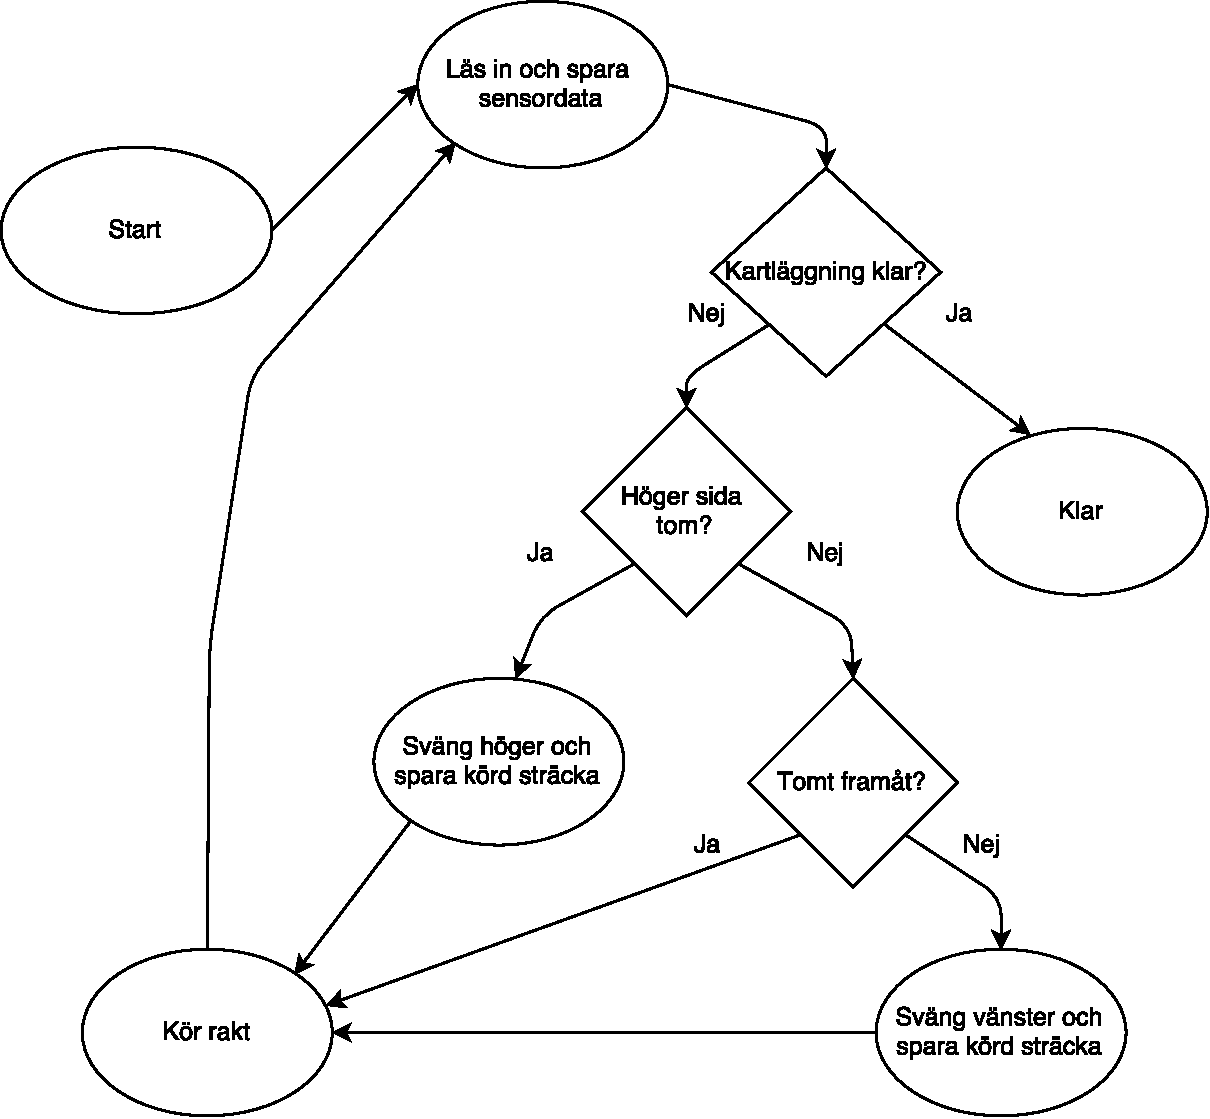
\includegraphics[scale=0.6]{navigering_flowchart}
\caption{Flödesdiagram för navigering.}
\label{fig:navigering_flowchart}
\end{figure}
\ \\

TODO:TEXT OM NAVIGERINGEN. FRÄMST OM KÖKSÖN OCH VÄNSTERREGLERING

\begin{figure}[H]
\centering

\includegraphics[scale=0.45]{Logo}
\caption{Flödesschema över Bluetooth-kommunikationen i huvudenheten.}
\label{fig:Kommunikation_huvudenhet_v2}
\end{figure}
\ \\

TODO:TEXT OM BLUETOOTH. UPPDATERA SÅ DEN REFLEKTERAR VÅR IMPLEMENTATION

\subsection{Sensorenhet}
% Se kommentarer för huvudenhet
TODO:TEXT OM SENSORENHET SOM REFLEKTERAR VÅR IMPLEMENTATION. LASER/GYRO ÄR T.EX PÅ BUSSEN DIREKT.

\subsubsection{Delsystemets funktion}
TODO:TEXT OM SENSORENHET SOM REFLEKTERAR VÅR IMPLEMENTATION. LASER/GYRO ÄR T.EX PÅ BUSSEN DIREKT.

\subsubsection{Kopplingsschema}
\begin{figure}[H]
\centering

\includegraphics[scale=0.6]{Logo}
\caption{Kopplingsschema för sensorenheten.}
\label{fig:sensorenhet_kopplingsschema}
\end{figure}

TODO:TEXT OM KOPPLINGSSCHEMA

\subsubsection{Komponenter}

TODO:DISKUTERA VAD SOM FAKTISKT LIGGER I SENSORENHETEN. LASER/GYRO ÄR LITE GRÅZON
\begin{table}[H]
  \centering
  \begin{tabular}{ | c | c | c | c |}
    \hline
    \textbf{Komponent} & \textbf{Antal} \\
    \hline
    ATMega 1284 & 1 \\
    \hline
    LIDAR-Lite v2 & 1 \\
    \hline
    Knapp & 1 \\
    \hline
    GP2Y0A41SK IR-Sensor & 2 \\
    \hline
    Adafruit 10-DOF IMU & 2 \\
    \hline
    EXO3 & 1 (delad) \\
    \hline
  \end{tabular}
  \caption{ Tabell över de komponenter som sensorenheten består av. }
\end{table}

\subsubsection{Resurser}
% Rada upp tillgängliga portar på mikroprocessorn samt hur många som krävs
% Motivera val av mikroprocessor med uppskattning av de resurser som krävs (prestanda, minne, IO)

TODO:TABELLEN NEDAN EJ KORRIGERAD
\begin{table}[H]
  \centering
  \begin{tabular}{ | c | c | c | c |}
    \hline
    \textbf{Port} & \textbf{Antal} & \textbf{Krävs} \\
    \hline
    SDA & 1 & 1 \\
    \hline
    SCL & 1 & 1 \\
    \hline
    PCINT & 24 & 1 \\
    \hline
    A/D & 8 & 2 \\
    \hline
    RESET & 1 & 1 \\
    \hline
    USART & 4 & 2 \\
    \hline
    JTAG & 1 & 1 \\
    \hline
    CLK & 1 & 1 \\
    \hline
  \end{tabular}
  \caption{Tabell över tillgängliga portar på processorn.}
\end{table}

TODO:TEXT FÖR MOTIVATION OM DESIGNBESLUT OCH RESURSUPPSKATTNING


\subsubsection{Programflöde}

\begin{figure}[H]
\centering

\includegraphics[scale=0.6]{Logo}
\caption{Ett flödesdiagram över sensorenhetens tillstånd}
\label{fig:sensorenhet_flowchart}
\end{figure}
TODO:TEXT OM PROGRAMFLÖDE SOM REFLEKTERAR IMPLEMENTATION

\subsection{Styrenhet}
% Se kommentarer för huvudenhet
TODO:UPPDATERA TEMPUS

\subsubsection{Delsystemets funktion}
TODO:UPPDATERA TEMPUS

\subsubsection{Kopplingsschema}
\begin{figure}[H]
\centering

\includegraphics[scale=0.45]{Logo}
\caption{Kopplingsschema för styrenheten.}
\label{fig:styrenhet_kopplingsschema}
\end{figure}

TODO:TEXT OM KOPPLINGSSCHEMA

\subsubsection{Komponenter}
TODO:TABELL NEDAN EJ KORRIGERAD
\begin{table}[H]
  \centering
  \begin{tabular}{ | c | c |}
    \hline
    \textbf{Komponent} & \textbf{Antal} \\
    \hline
    ATMega 1284 & 1 \\
    \hline
    Terminator (bas för fyrhjulingsrobot) & 1 \\
    \hline
    AX12-A Servo & 1 \\
    \hline
    EXO3 & 1 (delad) \\
    \hline
    LS241 & 1 \\
    \hline
  \end{tabular}
\end{table}


\subsubsection{Resurser}
TODO:TABELL NEDAN EJ KORRIGERAD
\begin{table}[H]
  \centering
  \begin{tabular}{ | c | c | c | c |}
    \hline
    \textbf{Port} & \textbf{Antal} & \textbf{Krävs} \\
    \hline
    SDA & 1 & 1 \\
    \hline
    SCL & 1 & 1 \\
    \hline
    RESET & 1 & 1 \\
    \hline
    IO & 30 & 5 \\
    \hline
    USART & 4 & 4 \\
    \hline
    JTAG & 1 & 1 \\
    \hline
    CLK & 1 & 1 \\
    \hline
  \end{tabular}
  \caption{Tabell över tillgängliga portar på processorn.}
\end{table}

Omvandlingen av kommandon från huvudenheten och utskickning av signaler till servona samt omhändertagandet och vidarebefodrandet av styrdata från servona till huvudenheten uppskattas ej kräva mer prestanda eller minne än styrenhetens ATMega 1284 processor klarar av.

\subsubsection{Programflöde}

\begin{figure}[H]
\centering

\includegraphics[scale=0.6]{Logo}
\caption{Ett flödesschema över styrenhetens tillstånd}
\label{fig:styrenhet_flowchart}
\end{figure}

TODO:TEXT SOM REFLEKTERAR IMPLEMENTATION

\subsection{Presentationsenhet}
% Se kommentarer för huvudenhet
TODO:UPPDATERA TEMPUS

\subsubsection{Delsystemets funktion}
TODO:UPPDATERA TEMPUS


\subsubsection{Blockschema}

% Övergripande schema för systemets stuktur
\begin{figure}[H]

\includegraphics[scale=0.37]{Logo}
\caption{Presentationsenheten i omgivning}
\label{fig:Oversikt_presentationsenhet3}
\end{figure}

TODO:TEXT OM BLOCKSCHEMA SOM REFLEKTERAR IMPLEMENTATION

\subsubsection{Komponenter}
Mjukvaruklienten och därmed presentationsenheten kräver en bärbar dator med Bluetooth. 


\subsubsection{Resurser}
TODO:VI ANVÄNDER INGEN TILLHANDAHÅLLEN BÄRBAR DATOR. KBRY?
Presentationen och behandlingen av datan som presentationsenhet mottager uppskattas ej kräva mer minne eller prestanda än vad den tillhandahållna bärbara datorn klarar av.

\subsubsection{Programflöde}
\begin{figure}[H]
\centering 

\includegraphics[scale=0.3]{Logo}
\caption{Flödesschema över presentationsenheten}
\label{fig:Presentationsenhet3}
\end{figure}

TODO:TEXT OM PROGRAMFLÖDE SOM REFLEKTERAR IMPLEMENTATION

\subsection{Fjärrstyrningsenhet}
% Se kommentarer för huvudenhet
TODO:TEXT SOM SPEGLAR IMPLEMENTATION

\subsubsection{Delsystemets funktion}
TODO:TEXT SOM SPEGLAR IMPLEMENTATION

\subsubsection{Blockschema}
% Övergripande schema för systemets stuktur
\begin{figure}[H]
\centering 

\includegraphics[scale=0.37]{Logo}
\caption{Fjärrstyrningsenheten i omgivning}
\label{fig:Oversikt_fjarrstyrenhet3}
\end{figure}
TODO:TEXT OM BLOCKSCHEMA SOM REFLEKTERAR IMPLEMENTATION

\subsubsection{Komponenter}
Fjärrstyrningsenheten kräver en dator med Bluetooth som kan köra mjukvaruklienten, samt tangentbord och mus/touchpad för interaktion med klienten. 

\subsubsection{Resurser}
TODO:VI ANVÄNDER INGEN TILLHANDAHÅLLEN BÄRBAR DATOR. KBRY?
Funktionaliteten för att ta emot användarinput och skicka iväg den via Bluetooth uppskattas ej kräva mer minne eller prestanda än vad den tillhandahållna datorn klarar av.


\subsubsection{Programflöde}
\begin{figure}[H]
\centering 

\includegraphics[scale=0.3]{Logo}
\caption{Flödesschema över fjärrstyrningssenheten}
\label{fig:Fjarrstyrningsenhet_flowchart3}
\end{figure}

TODO:TEXT OM PROGRAMFLÖDE SOM REFLEKTERAR IMPLEMENTATION

\section{Kommunikation mellan delsystem}
\label{sec:kommunikation_mellan_delsystem}
TODO:UPPDATERA TEMPUS, KANSKE IMPLEMENTATION?

\subsection{Huvudbuss}
TODO: KORREKTURLÄS SÅ DET FORTFARANDE STÄMMER 
Systemets moduler på roboten kommer vara sammankopplade med en I2C-buss (även kallad Two-Wire-Interface) där huvudenheten skickar och tar emot kommandon från sensor- och styrenheten. Huvudbussen kommer även att användas för att skicka sensordata från lasersensorn samt den kombinerade accelerometern och gyrot till sensorenhetens processor.

\subsubsection{Uppbyggnad}
TODO: KORREKTURLÄS SÅ DET FORTFARANDE STÄMMER 
Bussen består så som dess alternativa namn antyder av ett två-trådat gränssnitt och stödjer upp till 128 enheter. De två trådarna är SDA och SCL, där SDA överför data medan SCL styr med vilken frekvens detta sker. SDA kommer skrivas till utav bussens alla inkopplade enheter och behöver kopplas in till ett pull-up-motstånd för att inte flyta. Uppbyggnaden av bussen och dess master-slave förhållande kan ses i figur~\ref{fig:huvudbuss_masterslave}.

\subsubsection{Master-slave roller}
\begin{figure}[H]
\centering 

\includegraphics[scale=0.56]{Logo}
\caption{Huvudbussens uppbyggnad och master-slave förhållande}
\label{fig:huvudbuss_masterslave}
\end{figure}

TODO:UPPDATERA TEMPUS

\subsection{Bluetooth}
\label{sec:bluetooth}
TODO:UPPDATERA TEMPUS

\subsubsection{Handskakning}
\label{sec:handskakning}
\begin{figure}[H]
\centering 

\includegraphics[scale=0.8]{Logo}
\caption{Bluetooth mellan huvudenheten och mjukvaruklienten}
\label{fig:Kommunikation_Bluetooth}
\end{figure}

TODO:TEXT OM HANDSKAKNING SOM REFLEKTERAR IMPLEMENTATION

\subsubsection{Master-slave roller}
\label{sec:bluetooth_master_slave}
TODO:UPDATERA TEMPUS, KANSKE IMPLEMENTATION?

\subsection{Informationsflöde}
TODO:UPPDATERA TEMPUS

\subsubsection{Kommunikation med sensorenhet}
TODO:UPPDATERA TEMPUS

\subsubsection{Kommunikation med mjukvaruklient}
TODO:UPPDATERA TEMPUS

TODO:SE TILL ATT NEDANSTÅENDE LISTA SPEGLAR IMPLEMENTATION
Den data som skickas från mjukvaruklienten är följande
\begin{itemize}
\item Förfrågan om all ny kartdata sedan en viss tidpunkt t
\item Kommandon för att styra roboten
\item Byte av exekveringsläge
\end{itemize}
\ \\

TODO:SE TILL ATT NEDANSTÅENDE LISTA SPEGLAR IMPLEMENTATION
Den data som skickas till mjukvaruklienten är följande
\begin{itemize}
\item All ny kartdata sedan tidpunkt t
\item Kontinuerlig kartdata
\item Kontinuerlig mätdata
\item Kontinuerlig styrdata
\item Verifikation av kommandon
\end{itemize}

TODO:TEXT OM OVANSTÅENDE LISTOR

\nocite{*}
\bibliography{teknisk_dokumentation}{}
\bibliographystyle{plain}

TODO:BYT UT ALLA BILDER FRÅN PLACEHOLDERN LOGO OCH SE ÖVER ATT DE FORTFARANDE ÄR AKTUELLA
TODO:LCDn SKA IN NÅGONSTANS

\end{document}
